\section{Evaluation}\label{sec:eval}

In this section, we evaluate \name{}'s decentralized design and compare
with a state-of-the-art production workflow orchestrator---AWS Step
Functions---on latency and costs of running applications. Specifically, we ask
the following questions:

\begin{enumerate}

  \item Given the same application, what is the end-to-end latency of
    running it with \name{} and how does it compare with Step Functions?

  \item What are the sources of \name{'s} latency overhead? How much does
    the overhead come from API calls to the underlying serverless components?

  \item Given the same application, what is the billing cost of running it
  with \name{} vs that with Step Functions?

  \item What are the sources of \name{'s} billing costs? How much additional
  costs does the \name{} runtime incur in Lambda duration billing? And how
  much does it cost to provide exactly-once execution semantics from writing
  and reading checkpoints?

\end{enumerate}

% We show that 

% \begin{itemize}

  %     \item over 97\% of \name{}'s latency overhead comes from API calls to
  %     Lambda and data stores, which means the bulk of \name{}'s performance will
  %     automatically improve with the underlying platform (e.g., a faster Lambda
  %     or data store) without any modification to \name{} itself.

  %     % \item The additional Lambda duration billing for executing \name{} runtime
  %     % is negligible across all data sizes

  %     \item \name{} is slightly faster (11-28\%) in chaining performance and
  %     much faster in parallel fan-out and fan-in performance (up to 4.58x),
  %     especially at higher level of parallelism, than Step Functions.

  %     \item \name{} delivers more than one order-of-magnitude cost savings for
  %     almost all applications we evaluated, even when using the more expensive
  %     DynamoDB as the intermediary data store. The applications we use cover all
  %     orchestration patterns that Step Functions currently support.

  %     \item \name{} is able to express all orchestration patterns that Step
  %     Functions currently support. Additionally, with the ExCamera
  %     implementation, we demonstrate that \name{} can express fold or for loops
  %     and support pipeline parallelism, neither of which is expressible in Step
  %     Functions.

  % \end{itemize}

We use a combination of both microbenchmarks and 4 real-world applications,
for end-to-end analysis of \name{}. The micro-benchmarks target basic
orchestration patterns such as chaining, fan-out and fan-in
(\S\ref{sec:eval:micro}). The real-world apps consist of applications from
serverless repositories and prior research work  that encompass a variety of
orchestration patterns (\S\ref{sec:eval:realworld}).


\subsection{Experimental setup}

We run all experiments on AWS Lambda and DynamoDB in the same region,
\texttt{us-west-1}. All Lambda containers are configured with 128MB of memory
unless otherwise noted. We use on-demand capacity provisioning for DynamoDB.
Experiments that use Step Functions as baseline use Step Functions in the same
region, as well. To avoid performance artifacts related to cold-starts in
comparisons, we ensure all functions are warm by running each workflow several
times before taking measurements.

We wrote all but one applications as AWS Lambda functions and Step Function
state machines to driver those functions and either ran them directly for Step
Function experiments, or compiled them to \name{} IR first for \name{}
experiments. The notable exception is our \name{} and Step Functions
implementations of ExCamera, which differ due to a limitation in the AWS State
Language. As a result, the more efficient \name{} implementation is written
directly in \name{} IR instead of compiled from the Step Functions definition
(\S~\ref{sec:eval:realworld}).

For the Step Functions experiments, we run the workflow definitions using AWS
Step Functions in \emph{Standard}
configuration~\cite{aws-step-functions-standard-vs-express}, which provides
similarly strong execution guarantees as
\name{}~\cite{aws-step-functions-exec-gntee}.

In general, we treat Step Functions as a black box as its internal design or
implementation details are not public. While it is possible that different
designs for a centralized orchestrator could yield better performance, our
evaluation goal is merely to show that \name{}'s architecture and expression
language result in performance and cost sufficient for practical use. We argue
that if \name{} matches or improves over Step Functions, one of the most widely
used centralized orchestrators today, its performance and costs are good enough
for a wide variety of applications.

% We do not consider Step Functions' Express Workflows in our comparison because
% of its weaker execution guarantee, namely the same invocation could result in
% multiple and potentially diverging results if any part of the workflow logic
% is nonidempotent~\cite{aws-step-functions-exec-gntee}.

% Note that even though Step Functions claims that the Standard Workflows
% provides "exactly-once workflow
% execution"~\cite{aws-step-functions-exec-gntee}, it is not clear whether it
% implies exactly-once execution for component functions of the workflows. Our
% interpretation is that the internal states of a standard workflow will appear
% to execute exactly once, but component functions might not run exactly-once
% due to failures and retries, which is identical to \name{}. \shadi{this
  % paragraph is a bit confusing... }

\subsection{Performance}\label{sec:eval:micro}

\name{}'s performance overhead results from orchestration logic run in each
function as well as  storage and invocation APIs required to implement common
patterns. We characterize these overheads by measuring the latency to execute
various patterns in using \texttt{noop} functions as well as end-to-end
performance of real applications. Overall we find that \name{} performs
comparably or significantly better than Step Functions in most cases owing to
higher parallelism and a more expressive orchestration language, with modest
slow downs in the remaining cases due to implementation deficiencies.

\subsubsection{Chaining}

\begin{figure}[t]
  \centering
  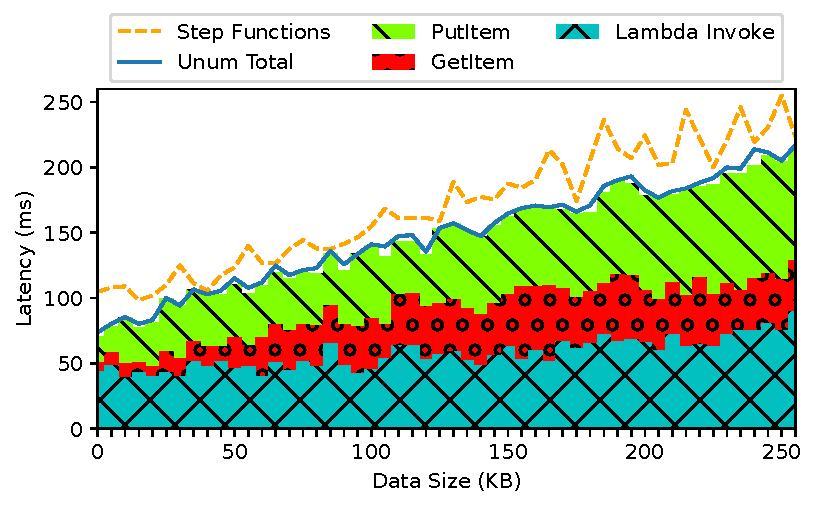
\includegraphics[width=\columnwidth]{figures/TotalAdditionalLatencyNBreakdown.pdf}
  \caption{An orchestrator incurs a latency on each transition between
functions. \name{}'s overhead is due to storage operations to ensure
exactly-once semantics, invocation API overhead to enqueue the next function to
run, and additional code running in the function instance itself for the
orchestration logic. \name{}'s overhead compares favorably to that of the Step
Function's orchestrator for simple, chain, transitions.}
  \label{fig:single-transition-latency-breakdown}
\end{figure}

For the simple chaining pattern, the \name{} runtime adds to each execution of a
function a storage write to checkpoint the function's result, a storage read to
find a previous checkpoint, and an asynchronous function invocation to initiate
the next function in the chain.

Figure~\ref{fig:single-transition-latency-breakdown} shows time to perform each
of these operations for different result sizes. As expected, storage operations
are slower when checkpointed results are larger, but the total overhead from the
\name{} runtime operations is consistently 50ms lower than an equivalent Step
Function transition.

\amit{We can keep Figure~\ref{chainmicrolatency} and explain briefly that this
basically confirms the thing, \emph{but} for that to be the case, it should be
the case that the difference between Step Functions and \name{} increases by
50ms for each additional link in the chain. Is this the case? Otherwise, I
think we can elide this figure.}

The \name{} implementation of the IoT pipeline application benefits from this
difference, with the \name{} version running 21\% faster than the Step Functions
version (Table~\ref{table:macro}).

%\subsubsection{Chaining performance}\label{sec:eval:chain}
%
%\emph{Highlight: Maybe just a repeat of the previous point with a different experiment}
%
%
%\begin{figure}[t]
%  \centering
%  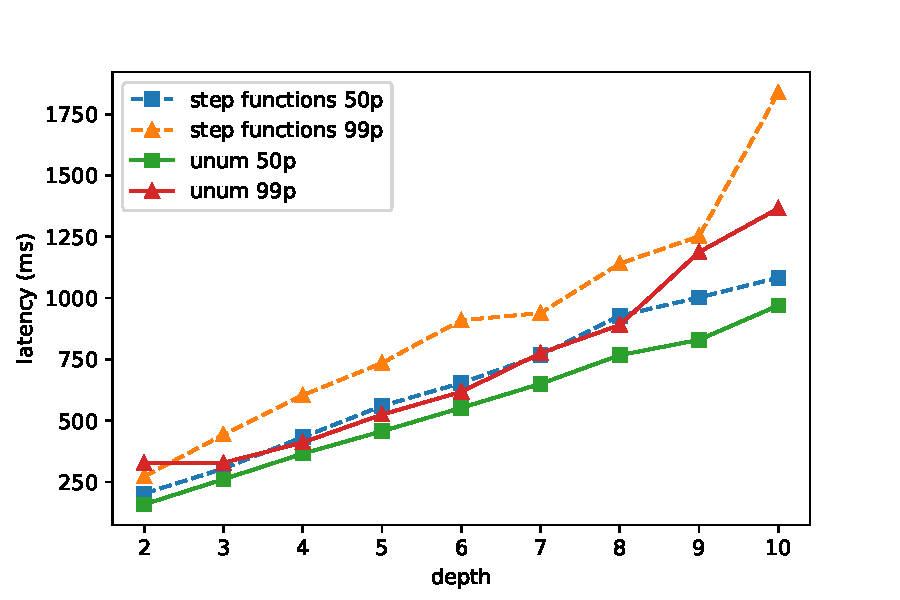
\includegraphics[width=\columnwidth]{figures/ChainMicroLatency.pdf}
%  \caption{End-to-end latency of chaining N functions. All constituent
%    functions in the experiment only run for 1-2ms, so the results mostly
%    reflect the latency of the workflow systems. \name{} is marginally
%    (11-28\%) faster than Step Functions on average. The results show that
%    \name{} is basically as fast in the most fundamental orchestration
%    primitive of transitioning from one function to the next.}
%  \label{fig:chainmicrolatency}
%\end{figure}
%
%
%We evaluate how \name{} performs on executing a series of functions in
%sequence and then compare with Step Functions. We measure the end-to-end
%latency of executing a chain of functions with varying chain lengths (2 to 10
%functions). Our goal is to allow the end-to-end latency to maximally reflect
%the performance of the workflow system, with minimum interference from the
%latency of user code. Therefore, we use a constituent function that simply
%returns its input without any computations to keep the user code runtime
%intentionally short (less than 2ms).
%
%Figure~\ref{fig:chainmicrolatency} shows the end-to-end latency of Step
%Functions and \name{} with DynamoDB. Overall, \name{} is around 43-173ms or
%11-28\% faster in chaining than Step Functions. A plausible explanation for
%the shorter latency is that a transition in \name{} from one function to the
%next involves a single network communication to Lambda when the source
%function calls the target function asynchronously. The same transition in Step
%Functions, however, requires not only an invocation from the orchestrator to
%Lambda but also a network communication from the source function to the
%orchestrator to send back the function output first. \name{} reduces
%the number of network communications because control-flow states and logic are
%decentralized to constituent functions without being managed by a centralized
%orchestrator.

\subsubsection{Fan-out and fan-in}\label{sec:eval:fan-out}

\emph{Highlight: fan-out doesn't require any additional storage; fan-in requires
additional reads and more expensive writes; compared to Step Functions, this
overhead results in slower fan-out/fan-in patterns at low branching factor;
conversely, \name{}'s parallelism is not limited by the orchestrator, so with
large branching factors, \name{} is much faster than Step Functions as fan-out
branches run in parallel.}

\begin{figure}[t]
  \centering
  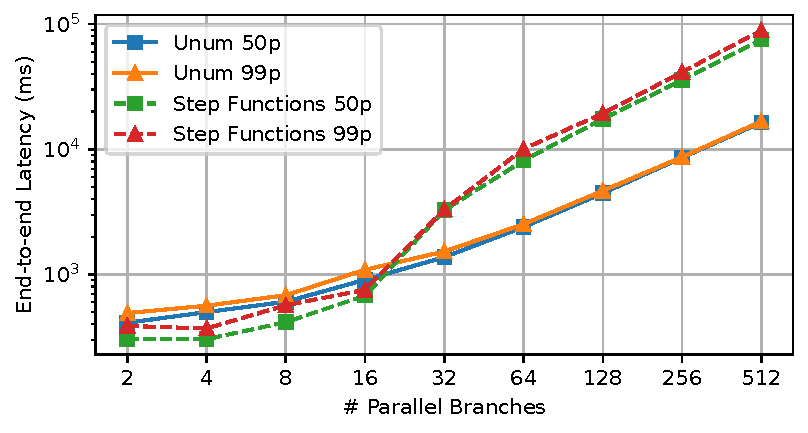
\includegraphics[width=\columnwidth]{figures/MapMicroLatency.pdf}
  \caption{End-to-end latency of a fan-out and fan-in pattern with increasing
branching degree. \name{} is 100-200ms slower at lower branching degrees due to
the distributed fan-in algorithm overhead. \name{} significantly outperform Step
Functions at moderate and high branching degree as the Step Function's
orchestrator is a scalability bottleneck for fan-out.}
  \label{fig:mapmicrolatency}
\end{figure}

Fan-out requires the same number of storage operations as chaining and similar
orchestration logic, but the \name{} runtime performs an additional asynchronous
invocation at the source function for each branch. For fan-in patterns, each
source branch performs an additional storage read to determine if it is the
final branch to execute, and only the final branch performs the asynchronous
invocation of the target function.

\amit{Why does \name{}'s latency grow at all in \ref{fig:mapmicrolatency}? If it
can do all branches in parallel, shouldn't latency remain roughly constant?}

Figure~\ref{fig:mapmicrolatency} shows the latency of a fan-out followed by a
fan-in at varying branching degrees for both \name{} and Step Functions. At low
branching degree, \name{}'s distributed fan-in algorithm incurs a modest
overhead (up to 200ms) relative to Step Functions. However, at higher branching
degrees (as low as 20 branches), Step Functions limits parallel invocation of
concurrent fan-out branches~\cite{aws-step-functions-map-state} while \name{} is
limited only by Lambda's scalability, resulting in over 4x lower latency with
512 branches.

These differences manifest in real workloads as well. Both the Text Processing
and Word Count applications include an fan-out followed by a fan-in. Text
Processing has low branching degree and, indeed, performs slightly worse on
\name{} than on Step Functions (1.8\%). Conversely, Word Count is highly
parallel and performs 219\% faster on \name{} than on Step Functions. (Table~\ref{table:macro})

% \subsubsection{Cost comparison}

% \begin{figure}[t]
  %     \centering
  %     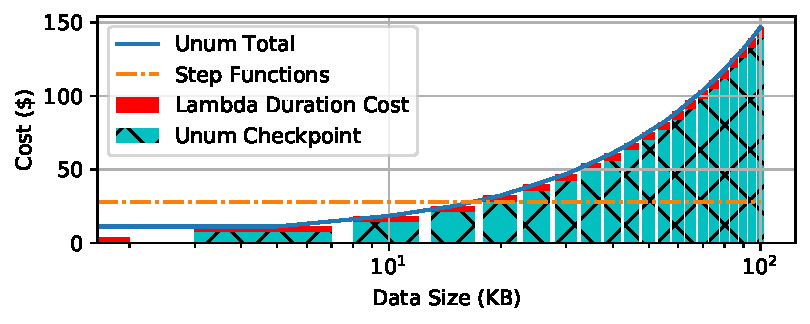
\includegraphics[width=\columnwidth]{figures/TotalCost.pdf}
  %     \caption{Total costs comparison of 1 million state transitions between
    %     Step Functions and \name{}. Computation assumes Lambda size of 3GB. \shadi{colors are hard to read}}
  %     \label{fig:total-costs-single}
  % \end{figure}

% \begin{figure}[t!]
  %     \centering
  %     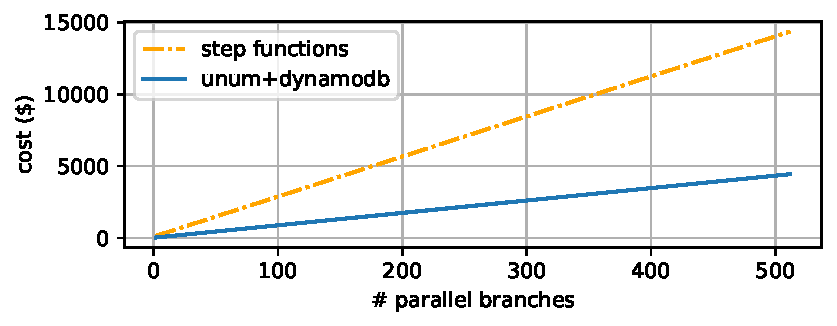
\includegraphics[width=\columnwidth]{figures/TotalMapCost.pdf}
  %     \caption{Total costs comparison of fan-out and fan-in between Step
    %     Functions and \name{}. Computation assumes Lambda size of 3GB and 1KB data
    %     size for function outputs and checkpoints.}
  %     \label{fig:total-costs-map}
  % \end{figure}

% In this section, we break down the cost of running workflows with \name{} and
% compare with that of Step Functions. We discuss the costs for a single transition,
% chaining and fan-out.

% Costs numbers are calculated based on AWS pricing for \texttt{us-west-1}
% region. We do not "measure" the cost of running workflows because AWS does not
% provide real-time billing data. We scale costs numbers by 1 million to ease
% reading.

% Step Functions charges based on the number of state
% transitions~\cite{aws-step-functions-pricing}. Each state transition is charged
% a fixed rate of \$27.9 $ \times 10^{-6}$.

% There are two parts to \name{}'s costs: (1). additional Lambda duration
% billing for running the \name{} runtime, and (2). data store reads and writes.

% We do not count the storage costs in the intermediary data store because after
% a workflow execution, checkpoints can be immediately deleted or moved to
% cheaper storage by the user.

% Figure~\ref{fig:total-costs-single} shows the total cost of transitions for
% function data size varying between 0-255KB. The computation assumes Lambda
% memory size of 3GB. We can see that the additional Lambda duration costs from
% running \name{} runtime is a small fraction when compared with the costs of
% DynamoDB writes. \shadi{how is the figure showing this? how do you translate lambda duration to cost in the figure? this figure is hard to understand. }
% In fact, even at 255KB, the additional Lambda
% duration costs is only abour \$10. If using the smallest 128MB lambdas \shadi{(instead of 3GB)}, the
% costs diminishes to merely \$0.46.

% DynamoDB writes dominates the costs in \name{} because the on-demand mode
% charges only not on the number of writes but also on the amount of data
% written. For 1KB of data, DynamoDB charges $1.3942 \times 10^{-6}$ for a write
% and $0.279 \times 10^{-6}$ for a read. Because checkpoint reads do not return
% any data when there are no faults, the cost of checkpoint reads does not
% increase with the data size and stays merely \$0.279 for the computation in
% Figure~\ref{fig:total-costs-single}.

% Even though the simulation in Figure~\ref{fig:total-costs-single} shows the
% costs of \name{} outpacing that of Step Functions at larger data sizes, our
% macrobenchmark results demonstrate that functions in real-world serverless
% workflows do not output large amount of data. In fact, workflows tend to use
% their own storage and manage application data manually. Checkpoints in the
% \name{} intermediary data store are normally under 1KB. 

% Figure~\ref{fig:total-costs-map} shows the total costs of fan-out and fan-in
% when function checkpoints are under 1KB. In addition to the costs discussed
% for a single transition, the entry function performing the fan-out incurs
% higher Lambda duration costs for invoking each fan-out function. The fan-in
% function at the end also causes extra costs because it reads the checkpoints
% of all fan-out branches. However, the total costs of this microbenchmark is
% more than 3.2x lower with \name{} than Step Functions.

% \begin{itemize}

  %     \item S3 charges \$5.5 per 1M PUT requests (for checkpoint write) and \$0.44
  %     per 1M GET requests (for checkpoint read).

  %     \item DynamoDB on-demand capcity mode charges reads and writes based on
  %     the data size. 1M requests for writing 1KB data costs \$1.3942 and 1M
  %     requests for reading 1KB data costs \$0.279. Note that in the case of
  %     DynamoDB, if no faults happen during execution, the checkpoint read will
  %     return "item not found", which costs the same as returning 1KB of data.

  %     \item For 1M state transitions, \name{}'s costs for S3:

  %     \[  r(d)\times0.05 + 5.94 \]

  %     and for DynamoDB:

  %     \[  r(d)\times0.05 + d\times1.3942 +0.279\],

  %     where $r$ is the total additional runtime of \name{}, $d$ is the data
  %     size.

  % \end{itemize}



\subsubsection{ExCamera}\label{sec:eval:excamera}

% \begin{table}[]
  % \begin{tabular}{llllll}
    % \hline
    %                      &                        & \multicolumn{2}{l}{\textbf{unum}}                                                                                                   & \multicolumn{2}{l}{\textbf{Step Functions}}                                                                     \\
    % \textbf{Application} & Pattern                & \textit{e2e latency} & \textit{cost (per 1M exec.)}                                                                                 & \textit{e2e latency} & \textit{cost (per 1M exec.)}                                                             \\ \hline
    % IoT Pipeline         & chain                  & 120.9ms              & $0.2*2+(73+28)*$0.0021+2*\$1.3942                                                                            & 226.52               & $0.2*2+ 4*$27.9                                                                          \\
    % Text Processing      & fan-out, fan-in        & 562.69ms             & $0.2*6+ (105+149+70+68+144+100)*$0.0021 + 6*$1.3942+2*2*$0.279                                               & 552.46ms             & $0.2*5+7*$27.9                                                                           \\
    % Wordcount            & chain, fan-out, fan-in & 410s                 & $0.2*(1+262+1+250+1) + (277+6264*262 + 348 + 667*250 +68)*$0.0021 +(1+262+1+250+1)*$1.3942 + 262*2*$0.279+ 250*2* $0.279    & 898s                 & $0.2*(1+262+1+250+1) + (5913*262 + 154 + 633*250 +5)*$0.0021 +(1+262+1+1+250+1+1)*\$27.9 \\
    % ExCamera             & chain, fan-out, fold   & 84s                  & $0.2*(1+16+15+15+14) + (6500+1500+350+4500+5000)*$0.0021+ (1+16+15+15+14)*$1.3942 + 15*2*$0.279+14*2*\$0.279 & 98s                  & $0.2*(16+16+1+16+15)+(6300+1400+2+5500+5300)*$0.0021+(1+16+16+1+1+16+1+1)*\$27.9      \\ \hline
    % \end{tabular}
  % \end{table}

\begin{table}[]
  \centering
  \begin{tabular}{|r|r|}
    \hline
    \textbf{ExCamera Implementation} & \textbf{Latency (seconds)} \\ \hline
    Original        & 76                         \\ \hline
    \name{} & 84                         \\ \hline
    gg                       & 90                         \\ \hline
    Step Functions & 98                         \\ \hline
  \end{tabular}
  \caption{\name{}'s implementation closely matches that of gg and the original
    ExCamera where a task starts as soon as its input data becomes available. The
    Step Functions implementation had to serialize the encoding and re-encoding
    stages because the \texttt{Map} state in Step Functions requires all parallel
    branches to complete before fan-in.}
  \label{table:excamera}
\end{table}

The ExCamera~\cite{excamera} video encoder applications encodes large raw videos
with thousands of concurrent functions. It breaks a large video into small
chunks and attempts to runs expensive steps in parallel and fast steps in
series. The original ExCamera design~\cite{excamera} used a custom centralized
orchestrator that implemented specialized workflow patterns which Step Functions
is unable to express efficiently.

The workflow consists of three stages, \texttt{ENCODE},
\texttt{ENCODE-GIVEN-STATE} and \texttt{REBASE}, where functions interact in
complex patterns. The first stage is a \texttt{map} that runs many
\texttt{ENCODE} functions entirely in parallel, the second stage forms paralllel
pipelines following the first stage where the $i^{th}$
\texttt{ENCODE-GIVEN-STATE} branch starts when the $(i)^{th}$ and $(i-1)^{th}$
\texttt{ENCODE} branch complete. The final \texttt{REBASE} runs in series and
rebases each chunk on top of the state from the previous chunk.

However, in Step Functions, all concurrent fan-out branches must complete before
any fan-in starts. As a result, a Step Functions implementation must serialize
the \texttt{ENCODE} and \texttt{ENCODE-GIVEN-STATE} stages.  Conversely,
\name{}'s IR is flexible enough to support ExCamera's original pattern where
tasks start as soon as their input data becomes available.

Table~\ref{table:excamera} compares the time to encode the first 888 chunks of
the \texttt{sintel-4k}~\cite{sintel-4k} video using 16 chunks per batch and
Lambdas configured with 3GB of memory in all cases.

%While ExCamera process all 888 chunks in parallel, each batch is a
%\texttt{map} with only 16 branches. From the result in
%\S\ref{sec:eval:fan-out}, we know that \name{} is around 200ms slower than
%Step Functions when launching 16 parallel branches. However, \name{} is able
%to win back 14.24s or 17\% of latency performance because fan-in in \name{} is
%wait-free. \name{} invokes the fan-in function whenever its input becomes
%available, whereas Step Functions first requires all branches to complete even
%if a branch is not part of the fan-in function's input, and lacks programming
%constructs to express fine-grained data dependencies between branches that can
%enable ``partial fan-in''.

\dhl{Sync with Design. Explain the difference between unum fan-in and Step
Functions fan-in in design already. Specifically,
inputs are available, whereas Step Functions fan-in first requires all
branches to complete even if a branch is not part of the fan-in function's
input.}

Table~\ref{table:excamera} compares \name{}'s implementation of ExCamera with
the original implementation and \texttt{gg}'s version. \name{}'s is 7.1\%
faster than gg and 10.5\% slower than the original ExCamera. The original
ExCamera pre-loads raw video chunks into lambdas before starting, while
\name{} and \texttt{gg} do not. The original authors attributes the
comparatively slower performance of \texttt{gg} to the lack of pre-loading
which is likely also the reason for \name{}'s slower performance. But
different from \texttt{gg}, \name{} executes control-flow logic in a
decentralized manner while \texttt{gg} has a centralized coordinator on EC2
that proxies inter-function communications and invokes lambdas. The reduced
number of network communications  explains why \name{} is slightly
faster than \texttt{gg}.


\subsection{Cost}

\begin{table*}[t]
  \centering
  \begin{tabular}{ll|rr|rr}
    \hline
    &                        & \multicolumn{2}{c}{\textbf{Latency (seconds)}}            & \multicolumn{2}{c}{\textbf{Cost (\$ per \emph{1 mil.} executions)}}       \\
    \textbf{Application} & \textbf{Pattern}       & \textit{\name{}} & \textit{Step Functions}   & \textit{\name{}} & \textit{Step Functions}            \\ \hline
    IoT Pipeline         & chain                  & 0.18       & 0.23       & 4.1       & 112.1   \\
    Text Processing      & fan-out, fan-in        & 0.56       & 0.55       & 12.0      & 196.3   \\
    Wordcount            & chain, fan-out, fan-in & 410.64     & 898.56     & 4,904.8   & 18,113.0 \\
    ExCamera             & chain, fan-out, fold   & 84.17      & 98.42      & 37,289.1   & 110,494.7      \\ \hline
  \end{tabular}
  \caption{Latency and costs comparison between \name{} and Step Functions for
    the macrobenchmark applications. Running applications on \name{} is 3.7x to
    32.8x cheaper than on Step Functions. Furthermore, \name{} is faster than Step
    Functions especially for workflows with high degrees of parallelism. Text
    Processing is the only workflow which \name{} is marginally slower because
    Step Functions creates parallel branches faster at low fan-out degrees as we
    illustrated in Figure~\ref{fig:mapmicrolatency}.}
  \label{table:macro}
\end{table*}

\begin{figure}[t!]
    \centering
    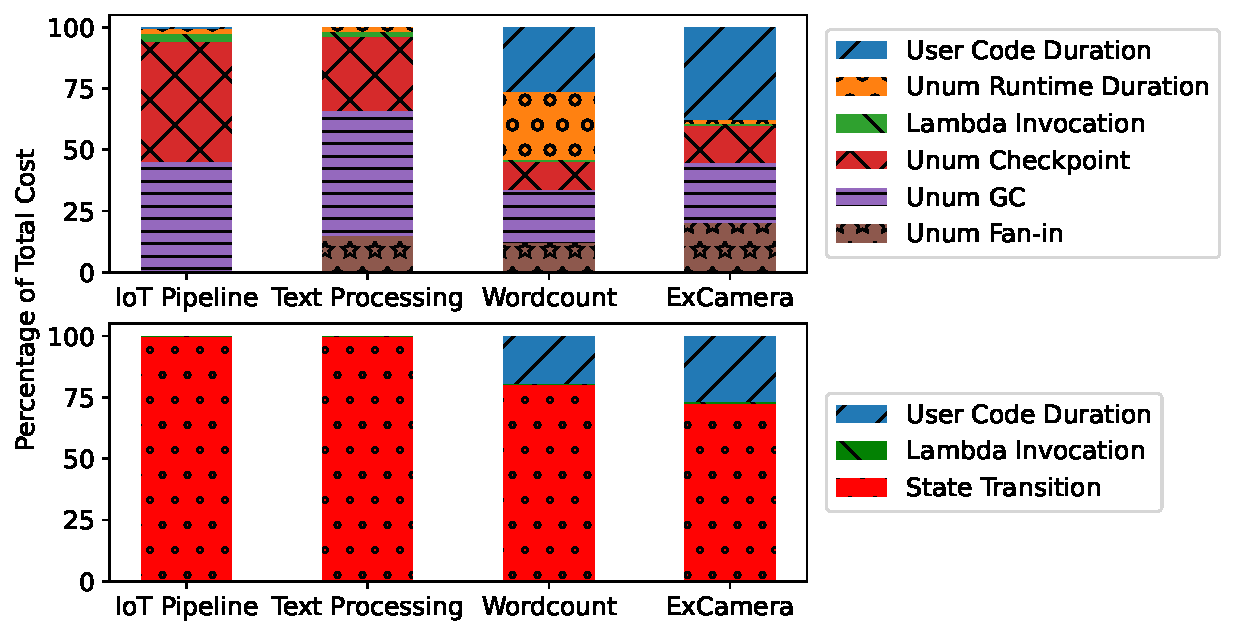
\includegraphics[width=\columnwidth]{figures/AppCostBreakdown.pdf}
    \caption{\dhl{I'm trying to figure out how the figure should look like. So
    trying a couple of things in this draft graph here. The top row splits
    \name{} breakdown and Step Functions breakdown to 2 graphs. The top left is
    the \name{} breakdown for just IoT Pipeline and Text Processing and no
    Wordcount or ExCamera. The top right is the Step Functions breakdown. The
    bottom row puts unum breakdown and Step Functions breakdown side-by-sdie.
    The bottom left is Wordcount and bottom right is ExCamera. Another
    thought: if percentage is the only thing we care about, should just pie
    charts instead? Esp. give that we already have Table~\ref{table:macro}.}
    \seb{I don't prefer pie charts. But i would perhaps normalize the cost 
    for each benchmark (e.g., define 1 = total cost of step functions) 
    and then put all 8 columns in a single double-tall chart. unum is going 
    to be a ridiculously short column but that may help to really make our point very visible.}
    Step Functions state transitions dominate the total costs of running
    applications, accounting for 72.2\% in ExCamera, 79.6\% in Wordcount and
    over 99\% in IoT Pipeline and Text Processing. While \name{} runtime and
    checkpoint costs are also the majority in IoT Pipeline (87.2\%) and Text
    Processing (89\%), for large-scale workflows, \name{} only accounts for
    18.1\% of the costs in ExCamera and 24.8\% in Wordcount. Most of \name{}'s
    costs come from reading and writing checkpoints to DynamoDB. A cheaper
    data store can significantly reduce the cost of using \name{}.}
    \label{fig:cost-breakdown}
\end{figure}

One of the main attractions of building appliactions on serverless platforms is
lower cost (or better resource utilization). In particular, because resources
are easy to reclaim, applications are charged only for resources used to respond
to actual events or requests. Thus, applications with potential for high
burst-parallelism, or with intermittant bursts of concurrent requests, can
achieve high performance without incurring the cost of long-term provisioning
for max capacity. As a result, the \emph{cost} of orchestration overhead matters
as well performance.

The source of costs for \name{} and Step Functions is quite different. Step
Functions imposes a cost to developers, in addition to running Lambda functions,
for each workflow transition. This abstracts the underlying, likely shared,
costs to run the Step Functions servers, persist state and checkpoint data.
Conversely, \name
incurs costs directly from those services: additional Lambda compute time and
DynamoDB storage on AWS.

Figure~\ref{fig:cost-breakdown} shows the cost to run each application using
\name{} broken down to each component: storage costs for checkpointing, Lambda
invocation, and Lambda CPU-time for both the \name{} runtime and user function.
Storage costs, using DynamoDB, are the largest portion of overall cost. The
majority of \name{}'s costs come from reading and writing checkpoints to
DynamoDB.

Nonetheless, \name{} is consistently cheaper than Step Functions for all
applications we tested. Table~\ref{table:macro} shows the price to run each of
the applications we implemented based on public pricing information for AWS in
the \texttt{us-west-1} region using \name{} and Step Functions.


%Table~\ref{table:macro} are calculated based on public pricing information for
%AWS \texttt{us-west-1} region. We do not ``measure'' the costs of running
%workflows because AWS does not provide real-time billing results for all
%services.
%
%For Step Functions, the total costs of running an application consists of i.
%Lambda duration billing for running user code, ii. Lambda invocation billing
%for starting functions and iii. Step Functions state transition
%charges~\cite{aws-step-functions-pricing}. Step Functions charges a fixed rate
%of \$27.9 $ \times 10^{-6}$ per state transition. A state transition equates
%to an edge in the workflow graph in the case of chaining and fan-out. But
%fan-in only counts as one state transition. Additionally, Step Functions adds
%a \texttt{Start} and \texttt{End} state to each workflow that counts towards
%state transitions.
%
%The total costs of running an application with \name{} consists of i. Lambda
%duration billing for running the \emph{unumized} functions, that is both the
%user code and \name{} runtime code, ii. Lambda invocation billing for starting
%functions, and iii. data store reads and writes for checkpoints. DynamoDB
%charges $1.3942 \times 10^{-6}$ for writing and $0.279
%\times 10^{-6}$ for reading 1KB of data. We do not count the costs of storing
%the data in DynamoDB because after a workflow execution, users can immediately
%delete the checkpoints or move them to cheaper storage.

%Step Functions state transitions dominate the total costs of running
%applications, accounting for 72.2\% in ExCamera, 79.6\% in Wordcount and over
%99\% in IoT Pipeline and Text Processing. While \name{} runtime and checkpoint
%costs are also the majority in IoT Pipeline (87.2\%) and Text Processing
%(89\%), for large-scale workflows, \name{} only accounts for 18.1\% of the
%costs in ExCamera and 24.8\% in Wordcount.
%
% A cheaper data store that supports strong consistency and
%conditional updates can significantly reduce the cost of using \name{}. For
%instance, Cosmos DB charges $0.279 \times 10^{-6}$ (or one fifth of the write
%cost of DynamoDB) per 1KB for both reads and writes~\cite{cosmosdb-pricing}.

%While pricing of a particular service can change based on a multitude of
%factors, the amount of developement efforts and the size of going workloads
%that has already gone into Lambda and multi-tenant storage systems likely
%means that they are much more resource efficient than a specialized
%orchestrator service such as Step Functions. The resource efficiency advantage
%is likely going to persist given the bigger pool of users and applications for
%Lambda and DynamoDB as they are more fundamental services. Therefore,
%\name{}'s cost benefits are likely going to continue and become even larger as
%FaaS systems and serverless data stores continue to improve.

Of course, developer-facing pricing does not necessarily reflect \emph{actual}
costs and is only a weak proxy for resource utilization. However, it is clear
that, in practice, \name{}'s overheads do not result in unreasonable costs and,
in fact, often results in lower costs to the developer than Step
Functions---AWS's native workflow orchestrator. This suggests that at least
applications that currently run on Step Functions could afford to run using
\name{} instead.

Moreover, \name{} costs benefits from improvements to underlying infrastructure
or different pricing schemes. For example, Azure's Cosmos DB provides similar
performance and consistency guarantees to DynamoDB but charges 5x less to
perform a write operation (the dominant constituent of \name{} storage cost on
AWS).

% \subsubsection{Questions}

% \begin{enumerate}

%     \item How do we evaluate and present execution guarantee? Anything to show
%      to convince our reader that it's correct?

%     \item How do we evaluate other benefits that stem from a simpler design
%      (the fact that unum gets rid of the needs for a separate orchestrator
%      service), such as resource management, required staffing and other
%      hosting costs? Further on the resource utilization point, do we want to
%      say that dollar costs of running applications is a reasonable enough
%      proxy to resource consumption and therefore lower price = less resource
%      consumption = better resource utilization?

%     \item Should we run experiments with S3 and present those numbers?

%     \item How to discuss the expressiveness advantage? Specifically,

%         Step Functions has no way to express a for loop or fold.

%         Step Functions has no way to express pipeline parallelism.

%         Step Functions fan-in needs to make sure the aggregate data doesn't exceed a
%         limit, unum automatically passes data in using pointers to the intermediary
%         data store.

% \end{enumerate}

